\section{Deep Reinforcement Learning}
	In this section the content of the two developed notebooks is discussed, mainly the theory behind \textit{DRL}\footnote{Deep Reinforcement Learning}. The reader gets to know the basic concept of software agents and RL, the deep learning aspect with the help of an exemplary neural net and work out the necessary formulas in order to translate the theory into code. Further the environment is introduced, which defines the problem, that the algorithm needs to solve and also holds all rules, which constrain the algorithm.  All the theory, explanations and code can be found in full length in the enclosed notebooks:
	\begin{enumerate}
		\item Deep Reinforcement Learning Beginners Tutorial (1) - Theory 
		\item Deep Reinforcement Learning Beginners Tutorial (2) - Practice
	\end{enumerate}

\subsection{The Software Agent}
	Before the topic of RL can be explained, some basics need to be addressed in order to clarify the following explanation.
	For this, the term of \textit{software agent} is introduced, which, as part of artificial intelligence, is basically a program, that acts self sufficient to solve a task.
	There are three important aspects an agent should fulfil. 
	First is autonomous action, which means that an agent needs to make decisions without external help.
	Further an agent needs to execute multiple actions to complete its task. 
	This property is called proactive.
	Last but not least, an agent has to be reactive, which means it reacts on changes in the environment it is in.
	An optional ability, for an agent like this, is self sufficient improvement. For this the agent builds up knowledge after repetitively doing its task and improves itself this way.\\
	Basically, the part of the agent, which controls its actions, can be filled with different algorithms. In this case, this will be an implementation of RL, which fits all requirements of an agent.

\subsection{Reinforcement Learning}
	Reinforcement Learning is considered one of the three machine learning paradigms, alongside supervised learning and unsupervised learning.
	The main goal of RL is to create an agent, which can navigate by actions in an environment in a way to maximize a representation of a cumulative reward.
	The environment is the space that contains the agent. 
	The environment is discussed in detail later on.
	In order to maximize the reward, the agent has to learn by trial and error which actions most likely lead to a reward and which lead to a penalty.
	After some training, the agent will use its knowledge to avoid previous mistakes.
	It still has to explore the environment, because otherwise it can not be sure if it actually finds the global maximum or is just stuck at a local one and if there might be a better chain of actions.
	If this is compared to the real world, this method of learning is pretty close the human learning. 
	If a person gets hurt for example, the person is more likely to try to avoid the situation in the future.
	Still curiosity or necessity leads humans to exploring and thus maybe getting them into danger, but in the best case, will lead them to some kind of positive reward, like food for example.\\
	
	\subsubsection{The Concept of RL}
		An agent is contained by an environment.
		A momentary snapshot of the environment is called state.
		A state contains all information at a certain point in time for example the position of the agent or enemies.
		There is a permanent exchange of information between the agent and its environment.
		The agent receives the actual state and has to choose an action based on its logic. Everything the agent can use to alter its environment is called an action.
		Executing an action changes the environment based on a certain set of rules.
		After executing an action the agents receives the new state and a reward, which helps to decide whether its decision leads to a positive result.
		A reward can also be negative.
		The main goal for the agent is to learn the best action for each state, so that it can maximize the reward.
		Basically, an environment is just a set of states.
		The agent can move between states by executing actions.
		A good example for an environment is the universe.
		Humans and other living beings are agents, moving in the world.
		All the time they have to look at their surroundings and choose an action like moving across the street or waiting until it is free.
		The laws of physics restrains them, take gravity for example.
		All living things receive rewards like getting hurt or feeling satisfied, that is how they evaluate the actions.
		The environment is constantly changing, so they have to revaluate their decisions and choose an action again. 
		The following picture shows the whole procedure:\\ 

		\begin{figure}[h!]
			\begin{center}
				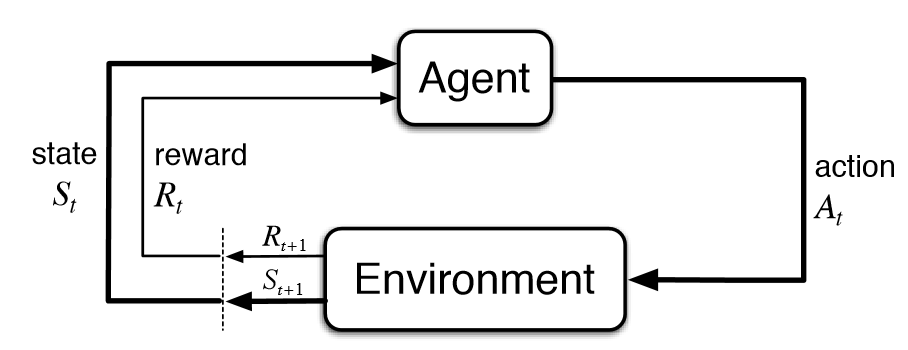
\includegraphics[width=0.7\linewidth]{img/eoeSq.png}
				\caption{Concept of Reinforcement Learning}
				\label{concept}
			\end{center}
		\end{figure}

	\subsubsection{Deep Learning Aspect}
		The agent has to recognize and differentiate elements in the environment, to be able to act accordingly and choose a proper action.
		In the best case, the input is already reduced to some important numbers, which describe the actual state.
		In real applications this may not be possible or feasible with the given knowledge.
		Most of the time there is a picture available, for example the image of a camera or a game screen, but the input the agent receives can basically be any sensory data.\\
		Furthermore the agent must associate the occurrence of individual elements on screen with its own actions and the subsequent reward or penalty, which may occur only after several steps in the future.
		Depending on the situation it may be also necessary to estimate what the next state of the game could be.
		There are two possible ways to use the \textit{deep learning} aspect.\\	
		\begin{enumerate}
			\item Image processing with a CNN\footnote{Convolutional Neural Network}, in order to process the image information and send this to the agent.
			\item A DQN\footnote{Deep Q-Learning Network}, in order to model the Q-function, which is discussed below.
		\end{enumerate}
		Following is an exemplary presentation of a neural network, which is designed according to the tasks just mentioned.
		\begin{figure}[h!]
			\begin{center}
				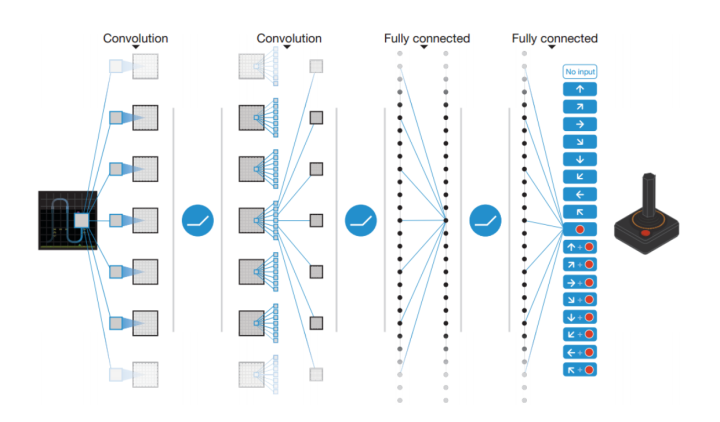
\includegraphics[width=0.7\linewidth]{img/v2-67ef75bb7f5e67b2a42645aa821894bf_hd.png}
				\caption{DQN with Convolutional Layers}
				\label{cnndqn}
			\end{center}
		\end{figure}\\
		There are two ways to learn in deep reinforcement learning.
		 Either the agent can use Value Learning or Policy Learning.
		 With Value Learning, it assigns values to each state-action pair, which correspond to the probabilities of the pair being the best option.
		 In Policy Learning, it will learn a strategy instead, which gives it directly the best estimated action for a given state s. 
		 In the notebook, the focus will be on Value Learning. 
			
	\subsubsection{Q-Learning}
		The task of the agent is the maximization of a cumulative future reward.
		An example of this can be the score in a game.
		In an environment, there is no guarantee for an immediate reward after executing an action.
		In many cases, only specific chains of actions lead to a positive reward, so the agent needs to learn multiple moves in succession in order to fulfil the given task.
		For example, if the agent needs to collect an object in order to get a higher score, it may be necessary to take multiple moves to reach it.
		The moves in between may not increase the reward significantly or even reduce it, however they are needed to complete the task in order to be successful.
		So the agent may have to learn to sacrifice some rewards, to earn an overall higher reward in the end.
		A simple way to implement RL is Q-Learning. A numerical value gets assigned to each action which can executed per state.
		This value is called Q-value.
		It represents an estimate of which action will result in the highest reward for the actual state.
		This is the knowledge of the agent.
		In the beginning all these values are initialized by 0.
		Each step the agent has to choose an action for the actual state.
		This is either random or knowledge based, but all the actions taken, provide data the agent is trained with.
		The agent uses random actions to explore its environment at first.
		If it uses its knowledge instead, the next action is chosen by exploitation, so the action with the highest Q-value for the given state is used.
		The next step is the associated function.
		The Q-function is the name giving aspect of a Deep Q-Learning Network, while the "Q" stands for "Quality".
		The higher the reward, the higher the estimated Q-value and associated quality.
		That means this function calculates a Q-value for the actual state, which represents the best action to take.
		Therefore taking the highest Q-value associated with the biggest estimated future total \textit{reward} $Q(s', a')$, the last gained reward and a discount factor into account is needed, in order to make rewards in the near future more decisive for the agent.
		The main formula to model such a behaviour is the so called \textit{Bellman equation}.
		
		\begin{figure}[h!]
			\begin{center}
				$Q(s_t, a_t) = r_t + \gamma * \max\limits_{a'} Q(s', a')$
			\end{center}
		\end{figure}